\FloatBarrier
\begin{figure}[!h]
\centering
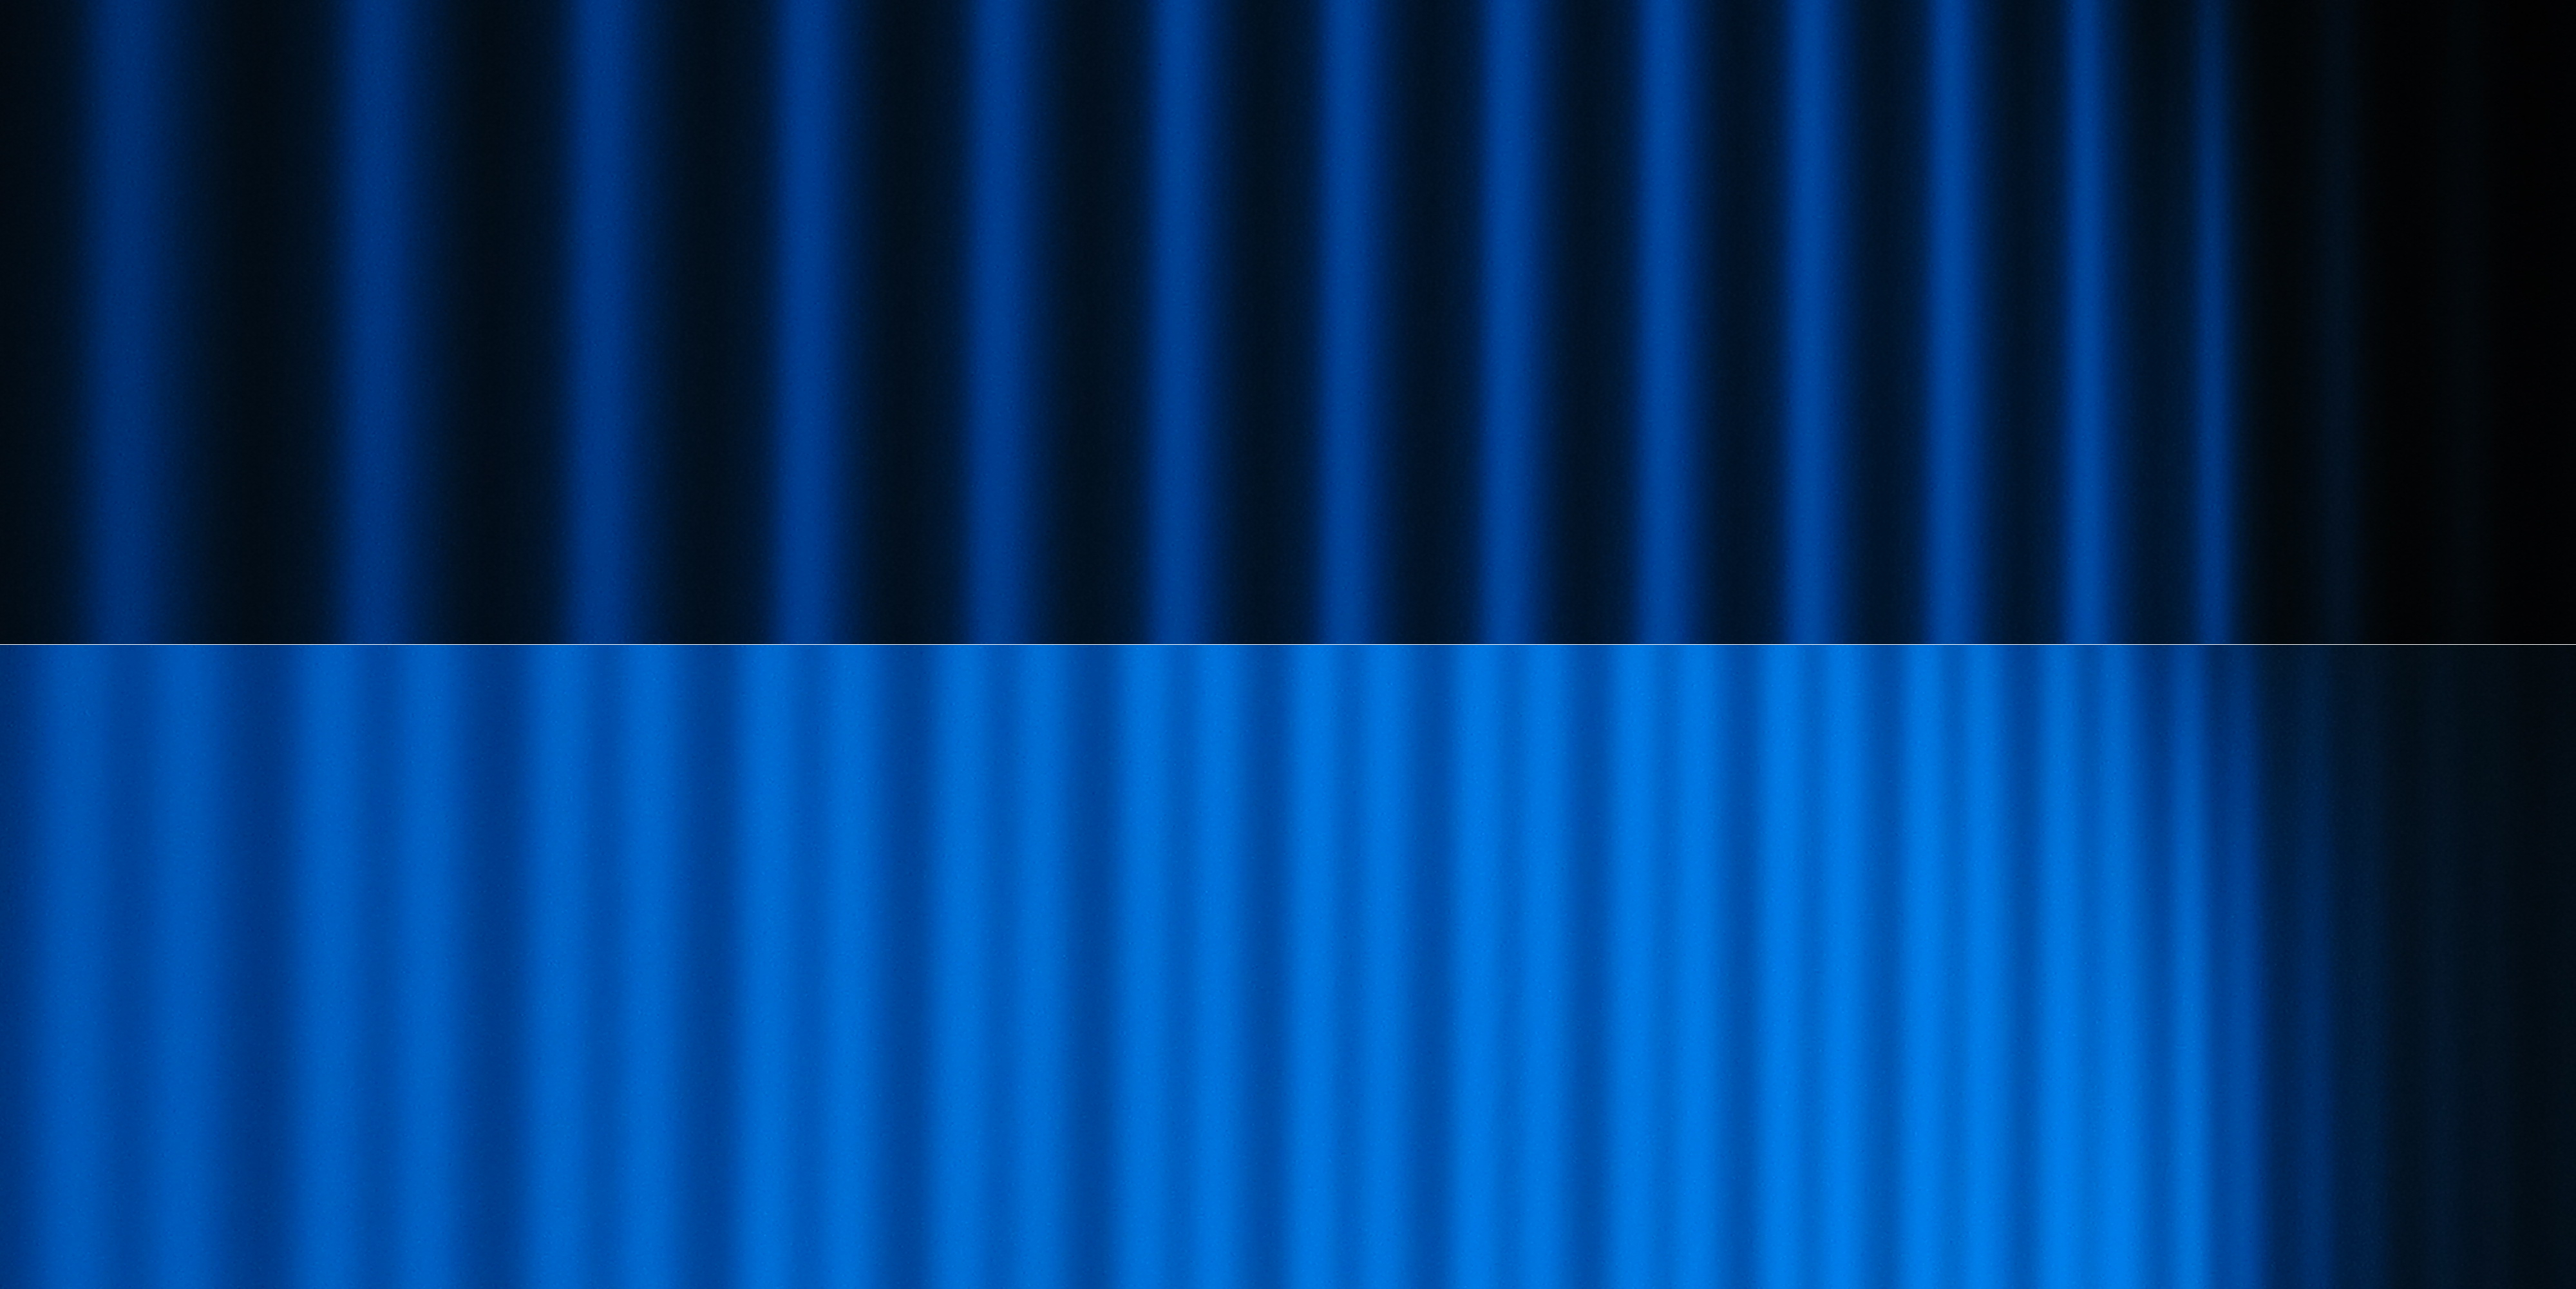
\includegraphics[scale=0.1]{../Grafiken/5-I0_t8_pi_6-I17_t8_pi.jpg}
\caption{Aufnahmen der roten $\pi$-Spekrallinie. Im oberen Teil ist die
        Spektrallinie ohne Einfluss eines äußeren Magnetfeldes abgebildet.
        Im unteren Teil ist die Zeemann-Aufspaltung der Spektrallinie
        im äußeren Magnetfeld zu erkennen.\label{fig:5-i0_t8_pi_6-i17_t8_pi}}
\end{figure}
\FloatBarrier
